\section{INTRODUCTION}
    \paragraph{}
    Optimizer is a critical component of a database system as it can optimize query execution plan to reduce database
    system execution time\cite{howgood}. Inside the optimizer, cardinality and cost estimation play 
    an important role in the process of optimization\cite{howgood}. Traditional approaches use statistic of tables to 
    do cost estimation and cardinality estimation\cite{Self-Tuning-Histograms,independenceisgood,lohman2014query}, 
    which cannot consider the relations between tables and columns in database instances\cite{howgood,lohman2014query}. 
    Consequently, the optimizers' estimation results are often inaccurate, which lead to the fail of selecting the optimal execution plan. 
    \paragraph{}
    Recent years have witnessed a growing academic interest in
    \cite{marcus2019neo, yang2020neurocard, wu2021unified, yang2019deep, sun2019end} the application of learning model 
    to database system optimization, especially the optimization of cardinality estimation. These work have greatly improved 
    accuracy of estimation results. 
    
    Most of the current work remain 
    at the level of cardinality estimation\cite{marcus2019neo, yang2020neurocard,wu2021unified,yang2019deep}
    and the improvement indicator is the reduction of estimation errors. However, better cardinality estimation does not imply better execution plan, which 
    directly affects the system's performance. There is few research that\cite{sun2019end}
    focus on improving performance of the database system beyond the scope of merely estimating cardinality and in an end-to-end manner. 
    
    In addition, to the best of the author's knowledge, all previous work take the stand-alone database instance as the testing environment and there is no  
    work for the distributed system, which is widely used nowadays and in urgent need of performance improvement.
    
    \paragraph{}
    Based on these two motivations, we set an ultimate goal of designing and implementing a learning-based query optimizer, and 
    integrating it to Hive\cite{Hive}, which is a well-known data warehouse software project and widely used in industry. 
    To progressively achieve the final goal, this paper dives into Hive system to fathom the mechanisms of Hive optimizer, such as how Hive optimizer performs 
    cardinality and cost estimation, how Hive optimizer performs join order selection and join algorithm selection. Moreover, a series of experiments are 
    conducted to evaluate the latent performance gain of learning-based optimizer in different benchmarks (e.g., Start Schema Benchmark and TPC-H), data scales, 
    query characteristics (e.g., join number) and different system configurations. The remaining part of this paper is organized as follows: section \ref{related_work} 
    introduces related work of learning-based optimizer; section \ref{hive-optimizer} illustrates the Hive optimizer; section \ref{experiments} finally shows results 
    and analysis of experimental studies.         

\section{RELATED WORK}\label{related_work}
    In this part, we review work that is most relevant to ours.
    \subsection{Traditional Cardinality Estimator}
    \paragraph{}
    \emph{Histogram-based} cardinality estimation methods\cite{Self-Tuning-Histograms} have been widely used in many 
    industrial database systems as they are simple and have very low overhead. However, they lack the ability to capture 
    the data correlations among the tables as they make the attribute-value-independence assumption. 
    \emph{Sampling-based} approaches\cite{Two-Level-Sampling} outperform histogram-based methods as the correlations 
    in data are naturally captured by data samples. However, sampling-based approaches have two limitations: (i) empty 
    sampling set of join result; and (ii) high sampling overhead. Recent work has proposed index-based and 
    materialized sampling strategies to alleviate the problem of empty result. However, it is still difficult to use 
    sampling to evaluate the cost of all execution plans as it incurs high space- and time- costs.
    
    \subsection{Learning-Based Cardinality Estimator}
    \paragraph{}
    Recently, the database community recognized the potential of replacing traditional cardinality estimation methods 
    by learning-based models (e.g., neural network, autoregressive model)\cite{Lan2021ASO}. Existing learning-based 
    estimators can be classified into three categories: query-driven, data-driven and hybrid\cite{wang2020we,wu2021unified}.
    \paragraph{}
    \textbf{Query-driven} cardinality estimators\cite{yang2019deep, yang2020neurocard, dutt2019selectivity} share the same idea with traditional 
    cardinality estimation methods, i.e., they hope to capture the correlations and distributions of data across the 
    tables. DeepDB\cite{yang2019deep} adopts relational sum product networks (RSPN) to capture the probability 
    distribution among relations, and translates a query into the evaluations of probabilities and expectations based 
    on RSPN. Naru\cite{naru2019} adopts autoregressive models, i.e., masked autoencoder and transformer to estimate 
    the selectivity of equal and range predicates. NeuroCard\cite{yang2020neurocard} trains a single deep autoregressive 
    model based on samples collected from the full outer join result of all relations. The model can be used to answer 
    complex queries with joins on any subset of the relations. 
    \paragraph{}
    \textbf{Data-driven} cardinality estimators\cite{deeplearningmodel20,sun2019end} formulate cardinality estimation as a 
    regression problem. The contents of queries and their true cardinalities are used as training data to learn a 
    mapping from queries to cardinalities. MSCN\cite{kipf2018learned} transforms a query into a feature vector and 
    uses a multi-set convolution network to map it to cardinality estimation. TLSTM processes a query execution plan
    recursively following its tree structure using LSTM (a kind of RNN).
    \paragraph{}
    \textbf{Hybrid} cardinality estimator UAE\cite{wu2021unified} learns the joint data distribution among the tables as in 
    the data-driven estimators, and uses query samples as auxiliary information at the same time. With a unified deep 
    autoregressive model, UAE learns from data in an unsupervised manner and query samples in a supervised manner. 

\section{HIVE QUERY OPTIMIZER}
\label{hive-optimizer}
    \paragraph{}
    To the best of our knowledge, there is no work about learning-based optimizer on distributed database systems. To implement a Learning-based optimizer 
    in distributed system, we should first study how distributed database system performs query optimization. Distributed database
    system (e.g., Hive, Spark) is much complicated than standalone database system (e.g., MySQL, PostgreSQL) because it needs to schedule
    several machines to complete a task together which involves storing data separately in several machines, dividing a task into subtasks 
    for machines and transferring data between machines. Hence it is harder to performs query optimization in distributed database systems than standalone
    database system. In this part, I will illustrate Hive optimizer from two aspects which are transformation and optimization of query in Hive Query Engine.

    \subsection{Query Transformation in Hive Query Engine}
        \paragraph{}
        We first focus on the transformation of query in Hive query engine. To meet users' habits in traditional standalone 
        database system, Hive supports users run SQL to process and access data in a distributed system. As the interface 
        between the database system and user, SQL will be converted to a physical execution plan which can be recognized
        by execution engine before execution. Figure 1, which is from paper of Hive, indicates the transformation of query.
        \begin{figure}[htb]
            \centering
            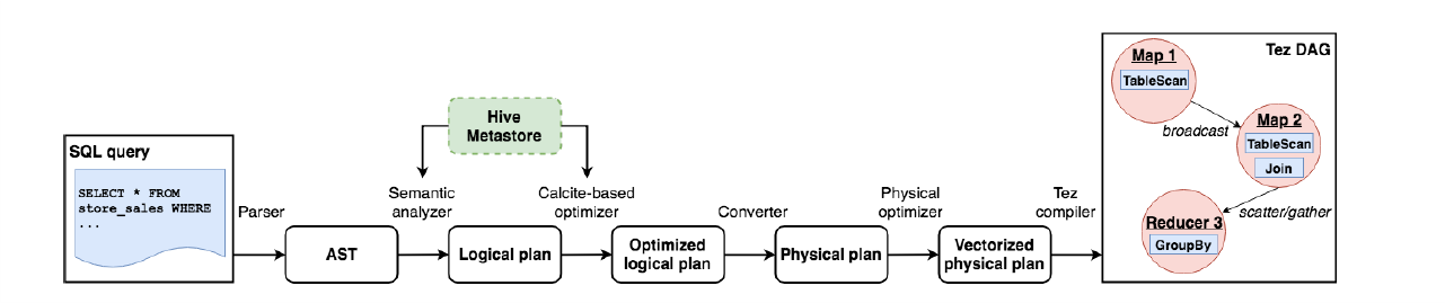
\includegraphics[width=1\textwidth]{figures/hive_mloptimizer/query_transformation.png}
            \caption{Query preparation stages in HiveServer2\cite{Hive}.}
            % 图片的标题应该在下方
        \end{figure}
        \paragraph{}
        This diagram illustrates the transformation of query in Hive query engine abstractly. It shows the physical implementation of each stage in code level. 
        SSB\cite{ssb} Q1.1 is taken as example.
        \paragraph*{SSB Q1.1}
        \begin{lstlisting}[language={SQL},%frame=shadowbox,    
            keywordstyle=\color{blue!30!black},  
            basicstyle=\ttfamily]  
        select 
            sum(lo_extendedprice*lo_discount) as revenue
        from 
            lineorder, dates
        where 
            lo_orderdate = d_datekey
            and d_year = 1993
            and lo_discount between 1 and 3
            and lo_quantity < 25;
        \end{lstlisting} 
        \paragraph{}
        At first, SQL is parsed as an abstract tree.
        \paragraph*{ASTree}
        \begin{lstlisting}[language={},%frame=shadowbox,    
            keywordstyle=\color{blue!30!black},  
            basicstyle=\ttfamily]  
(tok_query 
    (tok_from (tok_join 
        (tok_tabref (tok_tabname lineorder)) 
        (tok_tabref (tok_tabname dates)))
    ) 
    (tok_insert 
        (tok_destination (tok_dir tok_tmp_file)) 
        (tok_select (tok_selexpr (tok_function sum 
            (* 
                (tok_table_or_col lo_extendedprice) 
                (tok_table_or_col lo_discount)
            )) revenue)
        ) 
        (tok_where (and (and (and 
                (= 
                    (tok_table_or_col lo_orderdate) 
                    (tok_table_or_col d_datekey)
                ) 
                (= (tok_table_or_col d_year) 1993 )
            ) 
            (tok_function between kw_false 
                (tok_table_or_col lo_discount) 1 3)) 
            (< (tok_table_or_col lo_quantity) 25))
        )
    )
)
        \end{lstlisting}
        \paragraph{}
        Abstract Tree will be translated into an operator tree which is marked as logical plan in figure 1 by 
        Semantic Analyzer. Each node in the operator tree is an operator. Table scan short for TS,  which is 
        the operation that fetches data of table from disk, is always be the top nodes of a operator tree. This 
        logical plan has two tables scan operator as top nodes and two branches merge in the operator JOIN[8]. 
        The merged branch ends at the final file sink operator FS[15].
        \paragraph*{Logical plan}
        \begin{lstlisting}[language={SQL},%frame=shadowbox,    
            keywordstyle=\color{blue!30!black},  
            basicstyle=\ttfamily]  
    TS[0] - FIL[1] - SEL[2] - RS[6] - JOIN[8] - SEL[9] - SEL[10] - 
GBY[11] - RS[12] - GBY[13] - SEL[14] - FS[15]
    TS[3] - FIL[4] - SEL[5] - RS[7] - JOIN[8]
        \end{lstlisting}
        \paragraph{}
        Logical plan will be optimized by Hive cost-based optimizer which is implemented based on Calcite/cite{Calcite}. With an operator tree, 
        cost-based optimizer will match nodes of operator tree with many rewriting rules (e.g., PredicatePushDown, LimitPushDown) and rewrite matched nodes. 
        Besides rewriting operator tree, optimizer will also reorder join based on cost estimation which will be introduced in section \ref{section:cbo}.
        Optimized logical plan is following:
        \paragraph*{Optimized Logical plan}
        \begin{lstlisting}[language={SQL},%frame=shadowbox,    
            keywordstyle=\color{blue!30!black},  
            basicstyle=\ttfamily]  
    TS[0] - FIL[18] - SEL[2] - RS[6] - JOIN[8] - SEL[9] - GBY[11] - 
RS[12] - GBY[13] - FS[15]
    TS[3] - FIL[19] - SEL[5] - RS[7] - JOIN[8]
        \end{lstlisting} 
        \paragraph{}
        Comparing logical plan and optimized logical plan, it is obvious that FIL[1] and FIL[4] is replaced by 
        FIL[18] and FIL[19], redundant SEL[10] and SEL[14] are removed. Optimized logical plan will be converted
        into physical plan and DAG which are similar and we just show the summary graph of DAG.
        \paragraph*{DAG}
        \begin{lstlisting}[language={SQL},%frame=shadowbox,    
            keywordstyle=\color{blue!30!black},  
            basicstyle=\ttfamily]  
    Map 1 <- Map 3 (BROADCAST_EDGE)
    Reducer 2 <- Map 1 (CUSTOM_SIMPLE_EDGE)
        \end{lstlisting} 
        \paragraph{}
        In this DAG, node Map 1 and Map 3 will fetch data respectively from table \textbf{lineorder} and \textbf{dates} then 
        perform filtering operation. Once Map 3 finished processing data, it will broadcast data to node Map 1. 
        Map 1 will perform join and aggregate operation when it gets data from node Map 3 and send the result to 
        node Reducer 2. Reducer 2 will write the result to hive distributed file system. Here we have explained the query's transformation 
        in Hive query engine at the code level. Next, we will explain a more import issue in database system which 
        is query optimization.

    \subsection{Query Optimization in Hive Query Engine}
        \paragraph{}
        Hive query engine implements both of rule-based optimizer(RBO) and cost-based optimizer(CBO). Rule-based 
        optimizer optimizes query execution plan based on defined rules while cost-based optimizer optimizes query execution 
        plan based on cost estimation for different execution plans. Cardinality estimation is the foundation of 
        rule-based optimization and cost-based optimization because cardinality is needed to match rules in RBO and estimate 
        cost in CBO. Therefore, in this part, we will explain cardinality estimation, rule-based optimization and cost-based 
        optimization of Hive query engine.
        \subsubsection{Cardinality Estimation}
            \paragraph{}
            Cardinality estimation is to estimate the row count and size of output of intermediate operators which has a great
            effect on the optimization for execution plan. For instance, both of RBO and CBO reorder join operators and select 
            suitable join algorithm based on the cardinalities of input tables or intermediate tables. Seven operators (e.g., table 
            scan, select, filter, group by, join, limit, reduce sink) are implemented in Hive and only two of them (filter and 
            join operators) need to perform cardinality estimation. Cardinality estimation of filter operator cannot
            reach a high accuracy because of its assumption of uniform distribution. Cardinality estimation of join operators 
            cannot reach a stably accurate 
            estimation because rule-based cardinality estimation lacks the ability to capture the data correlations among the 
            tables as they make the attribute-value-independence assumption. Here we will explain the cardinality estimation methods 
            for filter and join operators in Hive query engine while these methods is referred to 
            \textit{Database Systems: The Complete Book}\cite{DatabaseSystems}.\\

            \textbf{Filter Operator}: Based on the assumption of uniform distribution of data\cite{DatabaseSystems}, cardinality 
            estimation result of equality comparison is the row count of table divided by the number of distinct values of the key 
            column. Assuming $R$ as a table, $x$ as the column to do filtering, $T(R)$ as the row count of 
            table, $V(R,x)$ as the number of distinct values of column $x$ and $S$ as the result table, 
            the result of cardinality estimation is \begin{equation}\label{equation_filter_cardinality_equality}
                T(S) = T(R) / V(R,x).
            \end{equation} For inequality comparison, based on the assumption
            that queries involving an inequality tend to retrieve a small fraction of the possible tuples and the typical
            inequality will return about one third of the tuples\cite{DatabaseSystems}, the result is 
            \begin{equation}\label{equation_filter_cardinality_inequality}
                T(S) = T(R) / 3.
            \end{equation}
            \textbf{Join Operator}: For join operator, we assume a simple join of two tables involves only the equality of two 
            columns and a more complicated join case can be drawn from this example. Assuming $X$, $Y$ as two tables
            to join and $x$, $y$ as key columns of $X$, $Y$ to join. The cardinality estimation result
            is \begin{equation}\label{equation_join_cardinality}
                T(S) = T(X)T(Y) / max(V(X,x), V(Y,y)).
            \end{equation}

        \subsubsection{Rule-based Optimizer}
        \label{section:rbo}
            \paragraph{}
            Rule-based optimizer in Hive optimizes execution plan based on defined rules which include rewriting rules and other rules. 
            Firstly, rule-based optimizer uses defined rewriting rules to match operator tree and rewrites matched operators iteratively 
            until no rewriting in last iteration. Rewriting rules help optimizer perform many basic but important optimizations, such
            as FilterPushDown, JoinReorder and removing redundant operators. 
            \paragraph{}
            In addition to the rewriting rules, rule-based optimizer also uses rules to do more like selecting the join algorithm 
            for each join operator. Hive implements two fundamental join algorithms which are map join and sort merge join. Hive processes
            data in MapReduce\cite{MapReduce} framework and all tasks are translated into MapReduce tasks to process. Map join can complete join
            in the map phase by buffering all data of a small table in the memory and streaming big table, hence reduce phase is not necessary.
            Therefore, map join usually runs faster than sort merge join. The selection of join algorithms is determined by the size of small table. In Hive
            default configurations, map join is used when the size of smaller table of two join tables is less than 10MB, otherwise, sort merge Join is used.             
            The boundary between a big table and a small table is modifiable and we have conducted related experiments.    
        
        \subsubsection{Cost-based Optimizer} 
        \label{section:cbo}
            \paragraph{}
            Similar to rule-based optimizer, cost-based optimizer also uses rewriting rules to perform basic optimization. What makes cost-based 
            optimizer different is that it could optimize query execution plan based on cost estimation. In hive cost-based optimizer, cost is computed 
            in terms of CPU usage, local IO usage, network IO usage, cardinality and size of tuple. Then I will introduce two vital optimizations in 
            Hive cost-based optimizer, join ordering and join algorithm selection. 
            \paragraph{}
            Join order has a great impact on the performance of query execution. Given a query, 
            Hive cost-based optimizer will generate a join tree via the following method:
            \newline
            (1) Generate a join tree for each table as root table, select the join tree with the least cost from all generated join trees;
            \newline
            (2) For a join tree with only a root table, optimizer will generate the join tree by inserting other tables into the join tree one by one;
            \newline
            (3) When selecting a table to insert into join tree, optimizer will select the table with the most cardinality = max(num(distinct values), max(value) 
            - min(value)).
            \newline
            (4) With a selected table, there are two ways (addToTop and pushDown) to insert the table into join tree, optimizer will select the generated join tree 
            with less cost. AddToTop means joining the selected table with the already generated join tree directly while pushDown means joining the selected 
            table with the corresponding join table in the already generated join tree first.
            \paragraph{}
            Hive cost-based optimizer mainly selects join algorithm from map join and sort merge join with the less cost. The cost of a join algorithm consists of three 
            dimensions which are row count of join tables, CPU cost and IO cost. The cost of map join and sort merge join can be estimated with the following method:
            \newline
            \newline
            \textbf{Map Join}
            \newline
            (1) Row count = Row count of the left table + Row count of the right table
            \newline
            (2) CPU cost = HashTable construction cost + Join cost
            \newline
            (3) IO cost = Cost of transferring small tables to join node * Degree of parallelism
            \newline
            \newline
            \textbf{Sort Merge Join}
            \newline
            (1) Row count = Row count of the left table + Row count of the right table
            \newline
            (2) CPU cost = Sorting cost of all tables + Merge cost
            \newline
            (3) IO cost = Cost of writing intermediary results to local FS + Cost of reading from local FS for transferring to join + Cost of transferring 
            map outputs to Join operator
    
    \paragraph{}
    In Hive query engine, both of rule-based and cost-base optimizers are applied to optimize query execution plan. To be specific, Hive generates join 
    tree via cost-based optimizer, selects join algorithms via rule-based optimizer and rewrites execution plan with rewrite rules of rule-based
    and cost-based optimizer. In this part, we first explain the query transformation in five stages at code level and then introduce query optimization from 
    cardinality estimation, rule-based optimizer and cost-based optimizer. So far, we have gained a comprehensive understanding of Hive's query optimization.

\section{EXPERIMENTAL STUDIES}
\label{experiments}
    \paragraph{}
    We conduct a series of experiments to evaluate the latent performance gain of learning-based optimizer on two benchmarks from 3 different aspects.
    (1) Latent performance gain of learning-based optimizer in different data scales. (2) Latent performance gain of learning-based optimizer on workload with 
    different query characteristics. (3) Latent performance gain of learning-based optimizer with different system configurations. 
    \subsection{Experiment Setting}
        \paragraph{}
        Experiments are conducted on a cluster of four machines all which are with 64GB RAM, 1.8TB disk, 2.4GHz CPU. Hive v3.1.0 is used.   
        \newline
        \textbf{Evaluation Techniques.} To evaluate the latent performance gain of learning-based optimizer, a best learning-based optimizer is simulated
        by feeding truth cardinality when Hive optimizer performs cardinality estimation. The reduction in execution time is taken as an indicator of performance 
        improvement. Because reduction in execution time may be caused by unstable cluster status, we also compare the query execution plan without truth 
        cardinality and plan with truth cardinality to validate performance improvement.
        \newline
        \textbf{Benchmarks.} Two benchmarks are used in this work. (1) Start Schema Benchmark\cite{ssb}, SSB for short. SSB has 5 tables (1 fact table, 4 dimension tables)
        and 13 queries. (2) TPC-H is a decision support benchmark. TPC-H has 8 tables and 22 queries. Both of SSB and TPC-H are commonly used benchmarks in performance 
        evaluation of distributed database system. Noted that due to the complexity of TPC-H queries, we only could feed truth cardinality in 8 TPC-H queries and they are 
        query 1, 3, 4, 6, 9, 10, 12 and 14.
        \newline
        \textbf{Data Scales.} Distributed database system needs to process data of the order of GB to EB, hence experiments are conducted to evaluate latent performance gain
        of learning-based optimizer in different data scales (5GB, 10GB, 50GB, 100GB). 
        \newline
        \textbf{Query Characteristics.} More joins in queries, more inaccurate cardinality estimation. Experiments are conducted to evaluate latent performance gain of 
        learning-based optimizer in workloads with different join numbers.
        \newline
        \textbf{System Configurations.} We have mentioned in section \ref{hive-optimizer} that join algorithms for joins are selected according to the size of smaller 
        table of two join tables. In Hive default configurations, map join is used when the size of smaller table is less than 10MB (system parameter Noconditiontasksize), 
        otherwise, sort merge join is used. Experiments are conducted to evaluate latent performance gain for learning-based optimizer 
        on system with different Noconditiontasksizes (e.g., 10MB, 50MB, 100MB, 150MB). 
    \subsection{Evaluate Latent Performance Gain of Learning-based Optimizer}
        \paragraph{}
        For each experiment scenario, we ran all queries of two benchmarks three or five times on initial Hive system and modified Hive system which feeds truth 
        cardinality during cardinality estimation, then averaged the collected execution time of each query as the its final execution time. For a 
        query $Q$, assuming $T_i$ as the final execution time of query in initial Hive system and $T_t$ as the final execution time of query in modified Hive 
        system, the latent performance gain \textit{PGain} of leaning-based optimizer is $$PGain(Q) = (T_i(Q) - T_t(Q)) / T_i(Q).$$ Because execution time of a query 
        is unstable due to the variation of cluster status, we take a performance improvement which is greater than 15$\%$ as a big performance improvement and a 
        performance degradation which is greater than 15$\%$ as a big performance degradation. We collected physical execution plans of those cases which have a big 
        performance improvement or performance degradation and studied what causes the performance variation.        
        \subsubsection{Different Data Scales}
            \paragraph{}
            We conducted experiments on two benchmarks in 4 data scales (5GB, 10GB, 50GB, 100GB) with default system configurations. Execution time of SSB 
            and TPC-H benchmarks in different data scales are shown separately in Table \ref{tab:scale_ssb_exectime} and \ref{tab:scale_tpch_exectime}. Performance 
            gain of SSB and TPC-H benchmarks in different data scales are shown in Table \ref{tab:scale_ssb_pgain} and \ref{tab:scale_tpch_pgain}. The performance 
            gain of cases which have a big performance improvement or performance degradation are bolded in Table \ref{tab:scale_ssb_pgain} and \ref{tab:scale_tpch_pgain}. 
            \paragraph{}
            We collected query execution plans of all cases with a big performance variation and summarized 3 main reasons for the observed big performance variations. (1) 
            Conversions of join algorithm between map join and sort merge join. In our experiment results, the conversions from sort merge join to map join always 
            improve the performance and the conversions from map join to sort merge join always degrade performance. (2) New join orders. Hive cost-based optimizer 
            generates join tree based on cardinality. Fed with truth cardinality, optimizer may generates a new join order for queries. In our experiment results, new 
            join order does not always improve performance. (3) Unstable cluster status. For a query, if the generated execution plan does not change fed truth 
            cardinality, the performance variation is caused by the variation of cluster status. The reasons of all cases with a big performance variation are shown in 
            Table \ref{tab:scale_pgain_reason}. 
            \paragraph{}
            From Table \ref{tab:scale_pgain_reason} and collected query execution plans, we have made some summaries:
            \newline
            (1) Most queries (16 of 21) don't have a true improvement variation for truth cardinality.   
            \newline 
            (2) New join order always has a continuity in different data scales while conversion between map join and sort merge join is limited by the data scales 
            (according to SSB queries Q2.2, Q3.1 and TPC-H query 9). Fed truth cardinality, SSB query Q3.1 in data scale as 100 and TPC-H query 9 in data scale as 5 
            also generate new join order. 
            \newline
            (4) \textbf{Larger latent performance gain in larger data scales} (according to SSB queries Q3.1, Q4.1 and Q4.3). 
            \newline 
            (5) \textbf{Hive's strategies of spanning join trees is not optimal}. Fed truth cardinality, Hive generates new execution plans with worse performance (according 
            to SSB queries Q4.1 and Q4.3).
               
            
% Please add the following required packages to your document preamble:
% \usepackage{booktabs}
% \usepackage{graphicx}
\begin{table}[]
    \caption{Execution Time of SSB Benchmark in Different Data Scales}
    \label{tab:scale_ssb_exectime}
    \small
    \centering
    \resizebox{\textwidth}{!}{%
    \begin{tabular}{@{}ccccccccc@{}}
    \toprule
    SSB Query & \multicolumn{2}{c}{Data Scale = 5}        & \multicolumn{2}{c}{Data Scale = 10}       & \multicolumn{2}{c}{Data Scale = 50}            & \multicolumn{2}{c}{Data Scale = 100}      \\ \midrule
              & \multicolumn{1}{c}{$T_i$ / s} & $T_t$ / s & \multicolumn{1}{c}{$T_i$ / s} & $T_t$ / s & \multicolumn{1}{c}{$T_i$ / s}      & $T_t$ / s & \multicolumn{1}{c}{$T_i$ / s} & $T_t$ / s \\ \midrule
    Q1.1      & 15.09     & 17.57     & 12.70     & 12.70     & 31.80          & 33.40     & 53.09     & 53.65     \\ 
    Q1.2      & 10.34     & 10.33     & 10.99     & 11.32     & 15.25          & 12.86     & 18.12     & 17.74     \\ 
    Q1.3      & 9.91      & 10.79     & 11.34     & 10.49     & 12.37          & 14.11     & 16.43     & 15.17     \\ 
    Q2.1      & 24.92     & 25.75     & 28.35     & 28.49     & 98.70          & 99.62     & 160.80    & 161.06    \\ 
    Q2.2      & 22.56     & 16.83     & 27.31     & 27.45     & 82.97          & 82.93     & 153.67    & 160.54    \\ 
    Q2.3      & 15.62     & 14.48     & 15.66     & 15.43     & 20.44          & 23.61     & 29.09     & 28.72     \\ 
    Q3.1      & 19.36     & 15.34     & 45.87     & 18.84     & 90.10          & 35.48     & 115.74    & 113.18    \\ 
    Q3.2      & 14.58     & 14.49     & 15.75     & 14.74     & 64.22          & 63.00     & 97.19     & 99.45     \\ 
    Q3.3      & 14.34     & 14.51     & 15.86     & 14.91     & 22.38          & 21.90     & 25.98     & 26.62     \\ 
    Q3.4      & 14.51     & 14.10     & 14.51     & 14.27     & 22.74          & 22.18     & 27.03     & 26.72     \\ 
    Q4.1      & 20.30     & 19.41     & 33.24     & 36.91     & 49.63          & 85.49     & 81.33     & 139.28    \\ 
    Q4.2      & 19.97     & 17.88     & 17.71     & 20.09     & 81.35          & 81.70     & 138.01    & 140.75    \\ 
    Q4.3      & 18.36     & 16.78     & 31.86     & 32.54     & 27.19          & 77.44     & 37.13     & 132.11    \\ 
    Total     & 219.86    & 208.26    & 281.13    & 258.20    & 619.12         & 653.72    & 953.63    & 1115.00   \\ \bottomrule
    \end{tabular}%
    }
    \end{table}

\begin{table}[]
    \caption{Execution Time of TPC-H Benchmark in Different Data Scales}
    \label{tab:scale_tpch_exectime}
    \centering
    \resizebox{\textwidth}{!}{%
    \begin{tabular}{@{}ccccccccc@{}}
    \toprule
    TPC-H Query & \multicolumn{2}{c}{Data Scale = 5}        & \multicolumn{2}{c}{Data Scale = 10}       & \multicolumn{2}{c}{Data Scale = 50}       & \multicolumn{2}{c}{Data Scale = 100}      \\ \midrule
                & \multicolumn{1}{c}{$T_i$ / s} & $T_t$ / s & \multicolumn{1}{c}{$T_i$ / s} & $T_t$ / s & \multicolumn{1}{c}{$T_i$ / s} & $T_t$ / s & \multicolumn{1}{c}{$T_i$ / s} & $T_t$ / s \\ \midrule
    1           & 10.99     & 11.01     & 11.35     & 11.54     & 42.65     & 22.73     & 31.14     & 25.12     \\ 
    3           & 21.60     & 20.11     & 26.44     & 22.77     & 52.21     & 48.88     & 90.11     & 85.07     \\ 
    4           & 18.44     & 19.38     & 20.47     & 20.39     & 33.85     & 33.50     & 43.40     & 54.46     \\ 
    6           & 9.06      & 9.90      & 9.62      & 9.07      & 12.21     & 12.54     & 17.32     & 16.08     \\ 
    9           & 37.26     & 35.63     & 44.64     & 62.00     & 120.18    & 148.49    & 222.32    & 259.68    \\ 
    10          & 17.62     & 19.10     & 20.87     & 22.23     & 37.83     & 39.50     & 67.44     & 84.81     \\ 
    12          & 14.29     & 14.50     & 15.94     & 16.14     & 29.00     & 28.68     & 44.73     & 65.71     \\ 
    14          & 11.78     & 13.28     & 13.02     & 14.76     & 18.24     & 19.83     & 26.57     & 30.33     \\ 
    Total       & 141.03    & 142.91    & 162.35    & 178.91    & 346.17    & 354.13    & 543.04    & 621.25    \\ \bottomrule
    \end{tabular}%
    }
    \end{table}

% Please add the following required packages to your document preamble:
% \usepackage{booktabs}
% \usepackage{graphicx}
\begin{table}[]
    \caption{Performance Gain of SSB Benchmark for Truth Cardinality in Different Data Scales}
    \label{tab:scale_ssb_pgain}
    \centering
    \resizebox{\textwidth}{!}{%
    \begin{tabular}{@{}ccccc@{}}
    \toprule
    SSB Query & Data Scale = 5  & Data Scale = 10 & Data Scale = 50  & Data Scale = 100 \\ \midrule
              & $PGain$ / \%    & $PGain$ / \%    & $PGain$ / \%     & $PGain$ / \%     \\ \midrule
    Q1.1      & \textbf{-16.43} & -0.02           & -5.03            & -1.07            \\ 
    Q1.2      & 0.10            & -3.01           & \textbf{15.69}   & 2.14             \\ 
    Q1.3      & -8.83           & 7.45            & -14.06           & 7.65             \\ 
    Q2.1      & -3.32           & -0.53           & -0.93            & -0.16            \\ 
    Q2.2      & \textbf{25.38}  & -0.53           & 0.04             & -4.47            \\ 
    Q2.3      & 7.33            & 1.43            & \textbf{-15.55}  & 1.26             \\ 
    Q3.1      & \textbf{20.75}  & \textbf{58.94}  & \textbf{60.62}   & 2.21             \\ 
    Q3.2      & 0.62            & 6.37            & 1.91             & -2.32            \\ 
    Q3.3      & -1.25           & 6.01            & 2.17             & -2.46            \\ 
    Q3.4      & 2.84            & 1.67            & 2.45             & 1.16             \\ 
    Q4.1      & 4.38            & -11.05          & \textbf{-72.27}  & \textbf{-71.25}  \\ 
    Q4.2      & 10.45           & -13.45          & -0.42            & -1.98            \\ 
    Q4.3      & 8.62            & -2.15           & \textbf{-184.84} & \textbf{-255.86} \\ 
    Total     & 5.27            & 8.16            & -5.59            & \textbf{-16.92}  \\ \bottomrule
    \end{tabular}%
    }
    \end{table}


% Please add the following required packages to your document preamble:
% \usepackage{booktabs}
% \usepackage{graphicx}
\begin{table}[]
    \caption{Performance Gain of TPC-H Benchmark for Truth Cardinality in Different Data Scales}
    \label{tab:scale_tpch_pgain}
    \centering
    \resizebox{\textwidth}{!}{%
    \begin{tabular}{@{}ccccc@{}}
    \toprule
    TPC-H Query & Data Scale = 5 & Data Scale = 10 & Data Scale = 50 & Data Scale = 100 \\ \midrule
                & $PGain$ / \%   & $PGain$ / \%    & $PGain$ / \%    & $PGain$ / \%     \\ \midrule
    1           & -0.22          & -1.67           & \textbf{46.71}  & \textbf{27.36}   \\ 
    3           & 6.88           & 13.88           & 6.39            & 5.59             \\ 
    4           & -5.11          & 0.36            & 1.05            & -6.50            \\ 
    6           & -9.33          & 5.64            & -2.66           & 7.16             \\ 
    9           & 4.37           & \textbf{-38.90} & \textbf{-23.56} & \textbf{-16.80}  \\ 
    10          & -8.38          & -6.52           & -4.41           & \textbf{-25.75}  \\ 
    12          & -1.46          & -1.21           & 1.09            & \textbf{-46.90}  \\ 
    14          & -12.71         & -13.34          & -8.70           & -14.15           \\ 
    Total       & -1.33          & -10.20          & -2.30           & -13.69           \\ \bottomrule
    \end{tabular}%
    }
    \end{table}

% Please add the following required packages to your document preamble:
% \usepackage{booktabs}
% \usepackage{multirow}
% \usepackage{graphicx}
\begin{table}[]
    \caption{Reasons to Big Performance Variations of Queries in Different Data Scales}
    \label{tab:scale_pgain_reason}
    \centering
    \resizebox{\textwidth}{!}{%
    \fontsize{20pt}{0}
    \begin{tabular}{@{}ccccc@{}}
    \toprule
    Benchmark              & Query                 & Data Scale & Performance Variation / \% & Reason of Performance Variation                                                                            \\ \midrule
    \multirow{11}{*}{SSB}  & Q1.1                  & 5          & -16.43                     & Unstable cluster status.                                                                                   \\  
                           & Q1.2                  & 50         & 15.69                      & Unstable cluster status.                                                                                   \\  
                           & Q2.2                  & 5          & 25.38                      & Conversion from sort merge join to map join.                                                              \\  
                           & Q2.3                  & 50         & -15.55                     & Unstable cluster status.                                                                                   \\ \cmidrule(l){2-5} 
                           & \multirow{3}{*}{Q3.1} & 5          & 20.75                      & New join order.                                                                                            \\  
                           &                       & 10         & 58.94                      & New join order.                                                                                            \\  
                           &                       & 50         & 60.62                      & New join order.                                                                                            \\ \cmidrule(l){2-5} 
                           & \multirow{2}{*}{Q4.1} & 50         & -72.27                     & New join order.                                                                                            \\  
                           &                       & 100        & -71.25                     & New join order.                                                                                            \\ \cmidrule(l){2-5} 
                           & \multirow{2}{*}{Q4.3} & 50         & -184.84                    & New join order.                                                                                            \\  
                           &                       & 100        & -255.86                    & New join order.                                                                                            \\ \midrule
    \multirow{7}{*}{TPC-H} & \multirow{2}{*}{1}    & 50         & 46.71                      & Unstable cluster status.                                                                                   \\  
                           &                       & 100        & 27.36                      & Unstable cluster status.                                                                                   \\ \cmidrule(l){2-5} 
                           & \multirow{5}{*}{9}    & 10         & -38.90                     & \begin{tabular}[c]{@{}c@{}}New join order.\end{tabular} \\  
                           &                       & 50         & -23.56                     & \begin{tabular}[c]{@{}c@{}}New join order and \\ conversion from map join to sort merge join.\end{tabular} \\  
                           &                       & 100        & -16.80                     & \begin{tabular}[c]{@{}c@{}}New join order and \\ conversion from map join to sort merge join.\end{tabular} \\ \cmidrule(l){2-5} 
                           & 10                    & 100        & -25.75                     & Unstable cluster status.                                                                                   \\  
                           & 12                    & 100        & -46.90                     & Unstable cluster status.                                                                                   \\ \bottomrule
    \end{tabular}%
    }
    \end{table}

    \subsubsection{Different Join Numbers}
        \paragraph{}
        Hive query optimizer estimates cardinality of joins via Equation \ref{equation_join_cardinality} and cannot consider the relations between tables 
        and columns in database, which would introduce error into cardinality estimation of joins. Moreover, errors of cardinality estimation of joins are superposed 
        during the process of join operations, which means more joins in queries may lead to greater error of cardinality estimation. Hence learning-based optimizer maybe has 
        a different latent performance gain in workloads with different join numbers. All queries of two benchmarks are sorted by the number of joins in Table 
        \ref{tab:join} and big performance variations due to truth cardinality are also noted in tables.
        \paragraph{}
        From Table \ref{tab:join}, we have made some summaries:
        \newline
        (1) Performance of queries with few joins (e.g., 0, 1, 2 joins) is not affected fed truth cardinality during query optimization. Few joins lead to small error
        of cardinality estimation, hence truth cardinality is not helpful in execution plan optimization.
        \newline
        (2) Queries with not many joins (e.g., 3 joins) could get performance gain fed truth cardinality. Queries with 3 joins have not complex join relations and 
        could get better execution plans due to truth cardinality.
        \newline
        (3) Queries with many joins (e.g., 4, 6 joins) in experiments only performance degraded. For these queries, Hive query optimizer generates not better or even worse 
        execution plans. We hold the opinion that Hive query optimizer maybe could not find optimal execution plans for queries with many joins.      

% Please add the following required packages to your document preamble:
% \usepackage{booktabs}
% \usepackage{multirow}
% \usepackage{graphicx}
\begin{table}[]
    \caption{Performance Variations of Queries with Different Join Numbers for Truth Cardinality }
    \label{tab:join}
    \centering
    \resizebox{\textwidth}{!}{%
    \begin{tabular}{@{}cccccc@{}}
    \toprule
    \multirow{2}{*}{Join Number} & \multirow{2}{*}{Query} & \multicolumn{4}{c}{Performance Variation for Truth Cardinality}                                                                                         \\ \cmidrule(l){3-6} 
                                 &                        & \multicolumn{1}{c}{Data Scale = 5}       & \multicolumn{1}{c}{Data Scale = 10}      & \multicolumn{1}{c}{Data Scale = 50}      & Data Scale = 100     \\ \midrule
    \multirow{2}{*}{0}           & TPC-H 1                & \multicolumn{1}{c}{}                     & \multicolumn{1}{c}{}                     & \multicolumn{1}{c}{}                     &                      \\  
                                 & TPC-H 6                & \multicolumn{1}{c}{}                     & \multicolumn{1}{c}{}                     & \multicolumn{1}{c}{}                     &                      \\ \midrule
    \multirow{6}{*}{1}           & TPC-H 4                & \multicolumn{1}{c}{}                     & \multicolumn{1}{c}{}                     & \multicolumn{1}{c}{}                     &                      \\  
                                 & TPC-H 12               & \multicolumn{1}{c}{}                     & \multicolumn{1}{c}{}                     & \multicolumn{1}{c}{}                     &                      \\  
                                 & TPC-H 14               & \multicolumn{1}{c}{}                     & \multicolumn{1}{c}{}                     & \multicolumn{1}{c}{}                     &                      \\  
                                 & SSB Q1.1               & \multicolumn{1}{c}{}                     & \multicolumn{1}{c}{}                     & \multicolumn{1}{c}{}                     &                      \\  
                                 & SSB Q1.2               & \multicolumn{1}{c}{}                     & \multicolumn{1}{c}{}                     & \multicolumn{1}{c}{}                     &                      \\  
                                 & SSB Q1.3               & \multicolumn{1}{c}{}                     & \multicolumn{1}{c}{}                     & \multicolumn{1}{c}{}                     &                      \\ \midrule
    2                            & TPC-H 3                & \multicolumn{1}{c}{}                     & \multicolumn{1}{c}{}                     & \multicolumn{1}{c}{}                     &                      \\ \midrule
    \multirow{8}{*}{3}           & TPC-H 10               & \multicolumn{1}{c}{}                     & \multicolumn{1}{c}{}                     & \multicolumn{1}{c}{}                     &                      \\  
                                 & SSB Q2.1               & \multicolumn{1}{c}{}                     & \multicolumn{1}{c}{}                     & \multicolumn{1}{c}{}                     &                      \\  
                                 & SSB Q2.2               & \multicolumn{1}{c}{\textbf{Improvement}} & \multicolumn{1}{c}{}                     & \multicolumn{1}{c}{}                     &                      \\  
                                 & SSB Q2.3               & \multicolumn{1}{c}{}                     & \multicolumn{1}{c}{}                     & \multicolumn{1}{c}{}                     &                      \\  
                                 & SSB Q3.1               & \multicolumn{1}{c}{\textbf{Improvement}} & \multicolumn{1}{c}{\textbf{Improvement}} & \multicolumn{1}{c}{\textbf{Improvement}} &                      \\  
                                 & SSB Q3.2               & \multicolumn{1}{c}{}                     & \multicolumn{1}{c}{}                     & \multicolumn{1}{c}{}                     &                      \\  
                                 & SSB Q3.3               & \multicolumn{1}{c}{}                     & \multicolumn{1}{c}{}                     & \multicolumn{1}{c}{}                     &                      \\  
                                 & SSB Q3.4               & \multicolumn{1}{c}{}                     & \multicolumn{1}{c}{}                     & \multicolumn{1}{c}{}                     &                      \\ \midrule
    \multirow{3}{*}{4}           & SSB Q4.1               & \multicolumn{1}{c}{}                     & \multicolumn{1}{c}{}                     & \multicolumn{1}{c}{\textbf{Degradation}} & \textbf{Degradation} \\  
                                 & SSB Q4.2               & \multicolumn{1}{c}{}                     & \multicolumn{1}{c}{}                     & \multicolumn{1}{c}{}                     &                      \\  
                                 & SSB Q4.3               & \multicolumn{1}{c}{}                     & \multicolumn{1}{c}{}                     & \multicolumn{1}{c}{\textbf{Degradation}} & \textbf{Degradation} \\ \midrule
    6                            & TPC-H 9                & \multicolumn{1}{c}{}                     & \multicolumn{1}{c}{\textbf{Degradation}} & \multicolumn{1}{c}{\textbf{Degradation}} & \textbf{Degradation} \\ \bottomrule
    \end{tabular}%
    }
    \end{table}
        
    \subsubsection{Different System Configurations}
        \paragraph{}
        Hive implements two main join algorithms map join and sort merge join. Map join loads all data of the smaller table of two join tables into memory and creates
        a hash table, then streams the data of larger table to perform join operation. Sort merge join first sorts the join key columns of two join tables in map phase 
        then performs join operation in reduce phase. Map join runs faster than sort merge join because map join can be completed in the map phase and reduce phase is not needed. 
        Hence map join should be used as much as possible to improve performance of Hive system. However, map join needs to put all data of a table into memory which is 
        unreachable if the size of table is larger than the storage of memory. Therefore, Hive has a system parameter \textbf{Noconditiontasksize}, with a default value
        as 10MB, to indicate how large a table is allowed to put all data into memory. If the size of smaller table is smaller than Noconditiontasksize, map join is 
        selected, otherwise sort merge join is selected. 
        \paragraph{}
        Default value of Noconditiontasksize is used in the previous experiments, which means sort merge join is selected when the size of smaller join table is greater
        than 10MB, even if the table size is only 11MB. A problem arises that whether 10MB is much small for the cluster while the size of a container of Hive is set 
        as 10GB. Experiments are conducted on SSB benchmark with data scale as 50, 100 and Noconditiontasksize as 50MB, 100MB, 150MB. Execution time of SSB benchmark 
        in data scale 50, 100 with different Noconditiontasksizes are shown in Table \ref{tab:noconditiontasksize_ssb_exectime_scale50} and 
        \ref{tab:noconditiontasksize_ssb_exectime_scale100}. Performance Gains of initial Hive for different Noconditiontasksizes, modified Hive for different 
        Noconditiontasksizes and Hive system with different Noconditiontasksizes for truth cardinality are shown in Table 
        \ref{tab:noconditiontasksize_ssb_pgain_scale50} and \ref{tab:noconditiontasksize_ssb_pgain_scale100}. 
        \paragraph{}
        From experiment results, we have mad some summaries:
        \newline{}
        (1) Both initial Hive system and modified Hive system benefit a lot from increase of Noconditiontasksize and total execution time of SSB benchmark in both 
        scale 50 and 100 decreases as the Noconditiontasksize increases. This is because when Noconditiontasksize increase, more sort merge joins are converted to 
        map join. When Noconditiontasksize is 150MB, initial Hive system got performance improvements of 64.56\% and 49.49\% in data scale 50, 100 while 
        modified Hive system got performance improvements of 67.92\% and 57.89\% in data scale 50, 100. 
        \newline{}
        (2) Noconditiontasksize cannot stably improve the latent performance gain of leaning-based optimizer. Hive system can benefit from the increased 
        Noconditiontasksize just because some sort merge joins are converted to map joins. Hence, truth cardinality can only improve the performance of
        such queries that has joins with truth cardinality less than Noconditiontasksize and estimated cardinality larger than Noconditiontasksize.
        \newline{}
        (3) Hive generate execution plans in an inappropriate manner. We can see SSB queries Q4.1 in data scale 50, 100 and Q4.3 in date 50 scale has no performance
        degradation when Noconditiontasksize is 150MB. However, Q4.1 and Q4.3 in data scale 50,100 has a great performance degradation when Noconditiontasksize is 10MB.
        As we mentioned in section \ref{hive-optimizer}, Hive generates join tree via cost-based optimizer and selects join algorithms via rule-based optimizer 
        and system configuration Noconditiontasksize is not considered in cost-based optimizer.
    
    \paragraph{}
    Experiments are conducted to evaluate the latent performance gain of learning-based optimizer in different benchmarks, different data scales, workloads with 
    different query characteristics and different system configurations. Some conclusions from experiment results: (1) Learning-based optimizer has \textbf{more latent
    performance gain in larger data scales}. (2) Learning-based optimizer has \textbf{largest latent performance gain in queries with medium join numbers}, has 
    \textbf{no latent performance gain in queries with few joins} and may has \textbf{latent performance degradation in queries with many joins}. (3) Increases of system configuration
    Noconditiontasksize can improve performance of Hive system but cannot stably improve latent performance gain of learning-based optimizer. (4) \textbf{Hive generates 
    execution plans in an inappropriate manner, which can be improved by combining join ordering and join algorithm selection}.
    
% Please add the following required packages to your document preamble:
% \usepackage{booktabs}
% \usepackage{multirow}
% \usepackage{graphicx}
\begin{table}[]
    \caption{Execution Time of SSB Benchmark with Different Noconditiontasksizes in Data Scale 50}
    \label{tab:noconditiontasksize_ssb_exectime_scale50}
    \centering
    \resizebox{\textwidth}{!}{%
    \begin{tabular}{@{}ccccccccc@{}}
    \toprule
    \multirow{2}{*}{SSB Query} & \multicolumn{4}{c}{$T_i$ / s}                                                                                 & \multicolumn{4}{c}{$T_t$ / s}                                                                                 \\ \cmidrule(l){2-9} 
                               & \multicolumn{1}{c}{size=10MB} & \multicolumn{1}{c}{size=50MB} & \multicolumn{1}{c}{size=100MB} & size=150MB & \multicolumn{1}{c}{size=10MB} & \multicolumn{1}{c}{size=50MB} & \multicolumn{1}{c}{size=100MB} & size=150MB \\ \midrule
    Q1.1                       & \multicolumn{1}{c}{31.80}     & \multicolumn{1}{c}{13.02}     & \multicolumn{1}{c}{10.91}      & 13.16      & \multicolumn{1}{c}{33.40}     & \multicolumn{1}{c}{13.06}     & \multicolumn{1}{c}{13.10}      & 13.24      \\ 
    Q1.2                       & \multicolumn{1}{c}{15.25}     & \multicolumn{1}{c}{12.56}     & \multicolumn{1}{c}{12.50}      & 12.71      & \multicolumn{1}{c}{12.86}     & \multicolumn{1}{c}{13.57}     & \multicolumn{1}{c}{13.25}      & 13.93      \\ 
    Q1.3                       & \multicolumn{1}{c}{12.37}     & \multicolumn{1}{c}{12.64}     & \multicolumn{1}{c}{13.41}      & 13.30      & \multicolumn{1}{c}{14.11}     & \multicolumn{1}{c}{14.30}     & \multicolumn{1}{c}{14.95}      & 9.92       \\ 
    Q2.1                       & \multicolumn{1}{c}{98.70}     & \multicolumn{1}{c}{67.45}     & \multicolumn{1}{c}{17.16}      & 17.99      & \multicolumn{1}{c}{99.62}     & \multicolumn{1}{c}{65.40}     & \multicolumn{1}{c}{15.72}      & 15.48      \\ 
    Q2.2                       & \multicolumn{1}{c}{82.97}     & \multicolumn{1}{c}{66.38}     & \multicolumn{1}{c}{64.66}      & 16.05      & \multicolumn{1}{c}{82.93}     & \multicolumn{1}{c}{17.98}     & \multicolumn{1}{c}{16.06}      & 14.39      \\ 
    Q2.3                       & \multicolumn{1}{c}{20.44}     & \multicolumn{1}{c}{18.71}     & \multicolumn{1}{c}{15.19}      & 13.14      & \multicolumn{1}{c}{23.61}     & \multicolumn{1}{c}{18.55}     & \multicolumn{1}{c}{13.45}      & 13.85      \\ 
    Q3.1                       & \multicolumn{1}{c}{90.10}     & \multicolumn{1}{c}{70.71}     & \multicolumn{1}{c}{23.17}      & 24.47      & \multicolumn{1}{c}{35.48}     & \multicolumn{1}{c}{28.16}     & \multicolumn{1}{c}{20.36}      & 18.27      \\ 
    Q3.2                       & \multicolumn{1}{c}{64.22}     & \multicolumn{1}{c}{17.99}     & \multicolumn{1}{c}{15.63}      & 14.29      & \multicolumn{1}{c}{63.00}     & \multicolumn{1}{c}{18.72}     & \multicolumn{1}{c}{13.26}      & 13.69      \\ 
    Q3.3                       & \multicolumn{1}{c}{22.38}     & \multicolumn{1}{c}{18.32}     & \multicolumn{1}{c}{15.18}      & 13.14      & \multicolumn{1}{c}{21.90}     & \multicolumn{1}{c}{17.87}     & \multicolumn{1}{c}{14.50}      & 14.44      \\ 
    Q3.4                       & \multicolumn{1}{c}{22.74}     & \multicolumn{1}{c}{18.21}     & \multicolumn{1}{c}{15.74}      & 13.01      & \multicolumn{1}{c}{22.18}     & \multicolumn{1}{c}{17.36}     & \multicolumn{1}{c}{14.22}      & 12.67      \\ 
    Q4.1                       & \multicolumn{1}{c}{49.63}     & \multicolumn{1}{c}{41.59}     & \multicolumn{1}{c}{25.39}      & 26.09      & \multicolumn{1}{c}{85.49}     & \multicolumn{1}{c}{80.38}     & \multicolumn{1}{c}{23.89}      & 24.81      \\ 
    Q4.2                       & \multicolumn{1}{c}{81.35}     & \multicolumn{1}{c}{25.55}     & \multicolumn{1}{c}{22.37}      & 22.28      & \multicolumn{1}{c}{81.70}     & \multicolumn{1}{c}{29.36}     & \multicolumn{1}{c}{24.06}      & 24.86      \\ 
    Q4.3                       & \multicolumn{1}{c}{27.19}     & \multicolumn{1}{c}{21.28}     & \multicolumn{1}{c}{22.99}      & 19.82      & \multicolumn{1}{c}{77.44}     & \multicolumn{1}{c}{73.45}     & \multicolumn{1}{c}{22.94}      & 20.17      \\ 
    Total                      & \multicolumn{1}{c}{619.12}    & \multicolumn{1}{c}{404.39}    & \multicolumn{1}{c}{274.31}     & 219.43     & \multicolumn{1}{c}{653.72}    & \multicolumn{1}{c}{408.14}    & \multicolumn{1}{c}{219.76}     & 209.73     \\ \bottomrule
    \end{tabular}%
    }
    \end{table}

% Please add the following required packages to your document preamble:
% \usepackage{booktabs}
% \usepackage{multirow}
% \usepackage{graphicx}
\begin{table}[]
    \caption{Execution Time of SSB Benchmark with Different Noconditiontasksizes in Data Scale 100}
    \label{tab:noconditiontasksize_ssb_exectime_scale100}
    \centering
    \resizebox{\textwidth}{!}{%
    \begin{tabular}{@{}ccccccccc@{}}
    \toprule
    \multirow{2}{*}{SSB Query} & \multicolumn{4}{c}{$T_i$ / s}                                                                                 & \multicolumn{4}{c}{$T_t$ / s}                                                                                 \\ \cmidrule(l){2-9} 
                               & \multicolumn{1}{c}{size=10MB} & \multicolumn{1}{c}{size=50MB} & \multicolumn{1}{c}{size=100MB} & size=150MB & \multicolumn{1}{c}{size=10MB} & \multicolumn{1}{c}{size=50MB} & \multicolumn{1}{c}{size=100MB} & size=150MB \\ \midrule
    Q1.1                       & \multicolumn{1}{c}{53.09}     & \multicolumn{1}{c}{20.91}     & \multicolumn{1}{c}{16.73}      & 22.68      & \multicolumn{1}{c}{53.65}     & \multicolumn{1}{c}{15.78}     & \multicolumn{1}{c}{11.21}      & 17.39      \\ 
    Q1.2                       & \multicolumn{1}{c}{18.12}     & \multicolumn{1}{c}{20.04}     & \multicolumn{1}{c}{17.53}      & 21.65      & \multicolumn{1}{c}{17.74}     & \multicolumn{1}{c}{15.81}     & \multicolumn{1}{c}{15.64}      & 18.30      \\ 
    Q1.3                       & \multicolumn{1}{c}{16.43}     & \multicolumn{1}{c}{24.72}     & \multicolumn{1}{c}{24.37}      & 19.70      & \multicolumn{1}{c}{15.17}     & \multicolumn{1}{c}{18.56}     & \multicolumn{1}{c}{16.52}      & 18.85      \\ 
    Q2.1                       & \multicolumn{1}{c}{160.80}    & \multicolumn{1}{c}{107.36}    & \multicolumn{1}{c}{110.86}     & 109.66     & \multicolumn{1}{c}{161.06}    & \multicolumn{1}{c}{109.13}    & \multicolumn{1}{c}{134.63}     & 106.17     \\ 
    Q2.2                       & \multicolumn{1}{c}{153.67}    & \multicolumn{1}{c}{105.49}    & \multicolumn{1}{c}{105.00}     & 101.88     & \multicolumn{1}{c}{160.54}    & \multicolumn{1}{c}{24.01}     & \multicolumn{1}{c}{34.21}      & 17.92      \\ 
    Q2.3                       & \multicolumn{1}{c}{29.09}     & \multicolumn{1}{c}{20.40}     & \multicolumn{1}{c}{19.90}      & 17.05      & \multicolumn{1}{c}{28.72}     & \multicolumn{1}{c}{22.46}     & \multicolumn{1}{c}{19.24}      & 17.70      \\ 
    Q3.1                       & \multicolumn{1}{c}{115.74}    & \multicolumn{1}{c}{90.81}     & \multicolumn{1}{c}{89.70}      & 33.97      & \multicolumn{1}{c}{113.18}    & \multicolumn{1}{c}{100.24}    & \multicolumn{1}{c}{100.13}     & 20.97      \\ 
    Q3.2                       & \multicolumn{1}{c}{97.19}     & \multicolumn{1}{c}{21.30}     & \multicolumn{1}{c}{15.82}      & 15.50      & \multicolumn{1}{c}{99.45}     & \multicolumn{1}{c}{22.59}     & \multicolumn{1}{c}{15.76}      & 18.94      \\ 
    Q3.3                       & \multicolumn{1}{c}{25.98}     & \multicolumn{1}{c}{19.53}     & \multicolumn{1}{c}{15.72}      & 13.70      & \multicolumn{1}{c}{26.62}     & \multicolumn{1}{c}{22.33}     & \multicolumn{1}{c}{16.33}      & 15.61      \\ 
    Q3.4                       & \multicolumn{1}{c}{27.03}     & \multicolumn{1}{c}{21.94}     & \multicolumn{1}{c}{17.43}      & 18.38      & \multicolumn{1}{c}{26.72}     & \multicolumn{1}{c}{17.71}     & \multicolumn{1}{c}{19.15}      & 19.26      \\ 
    Q4.1                       & \multicolumn{1}{c}{81.33}     & \multicolumn{1}{c}{59.62}     & \multicolumn{1}{c}{52.84}      & 44.21      & \multicolumn{1}{c}{139.28}    & \multicolumn{1}{c}{126.74}    & \multicolumn{1}{c}{137.99}     & 37.19      \\ 
    Q4.2                       & \multicolumn{1}{c}{138.01}    & \multicolumn{1}{c}{128.61}    & \multicolumn{1}{c}{28.03}      & 33.89      & \multicolumn{1}{c}{140.75}    & \multicolumn{1}{c}{124.51}    & \multicolumn{1}{c}{29.90}      & 31.25      \\ 
    Q4.3                       & \multicolumn{1}{c}{37.13}     & \multicolumn{1}{c}{28.39}     & \multicolumn{1}{c}{27.84}      & 29.43      & \multicolumn{1}{c}{132.11}    & \multicolumn{1}{c}{124.33}    & \multicolumn{1}{c}{126.59}     & 130.00     \\ 
    Total                      & \multicolumn{1}{c}{953.63}    & \multicolumn{1}{c}{669.11}    & \multicolumn{1}{c}{541.77}     & 481.70     & \multicolumn{1}{c}{1115.00}   & \multicolumn{1}{c}{744.21}    & \multicolumn{1}{c}{677.29}     & 469.54     \\ \bottomrule
    \end{tabular}%
    }
    \end{table}

% Please add the following required packages to your document preamble:
% \usepackage{booktabs}
% \usepackage{multirow}
% \usepackage{graphicx}
\begin{sidewaystable}[]
    \caption{Performance Gain of SSB Benchmark with Different Noconditiontasksizes in Data Scale 50}
    \label{tab:noconditiontasksize_ssb_pgain_scale50}
    \centering
    \resizebox{\textwidth}{!}{%
    \begin{tabular}{@{}ccccccccccc@{}}
    \toprule
    \multirow{2}{*}{SSB Query} & \multicolumn{3}{c}{\begin{tabular}[c]{@{}c@{}}Performance Variation of $T_i$ \\ Compared with size=10MB / \%\end{tabular}} & \multicolumn{3}{c}{\begin{tabular}[c]{@{}c@{}}Performance Variation of $T_t$ \\ Compared with size=10MB / \%\end{tabular}} & \multicolumn{4}{c}{\begin{tabular}[c]{@{}c@{}}Performance Gain for Truth \\ Cardinality\end{tabular}}                                                 \\ \cmidrule(l){2-11} 
                               & \multicolumn{1}{c}{size=50MB}                 & \multicolumn{1}{c}{size=100MB}                & size=150MB                & \multicolumn{1}{c}{size=50MB}                 & \multicolumn{1}{c}{size=100MB}                & size=150MB                & \multicolumn{1}{l}{size=10MB}        & \multicolumn{1}{l}{size=50MB}        & \multicolumn{1}{l}{size=100MB}      & \multicolumn{1}{l}{size=150MB} \\ \midrule
    Q1.1                       & \multicolumn{1}{c}{\textbf{59.07}}            & \multicolumn{1}{c}{\textbf{65.70}}            & \textbf{58.61}            & \multicolumn{1}{c}{\textbf{60.90}}            & \multicolumn{1}{c}{\textbf{60.77}}            & \textbf{60.34}            & \multicolumn{1}{c}{-5.03}            & \multicolumn{1}{c}{-0.34}            & \multicolumn{1}{c}{\textbf{-20.14}} & -0.65                           \\ 
    Q1.2                       & \multicolumn{1}{c}{\textbf{17.65}}            & \multicolumn{1}{c}{\textbf{18.02}}            & \textbf{16.66}            & \multicolumn{1}{c}{-5.50}                     & \multicolumn{1}{c}{-3.01}                     & -8.29                     & \multicolumn{1}{c}{\textbf{15.69}}   & \multicolumn{1}{c}{-8.01}            & \multicolumn{1}{c}{-5.94}           & -9.55                           \\ 
    Q1.3                       & \multicolumn{1}{c}{-2.16}                     & \multicolumn{1}{c}{-8.42}                     & -7.54                     & \multicolumn{1}{c}{-1.34}                     & \multicolumn{1}{c}{-5.99}                     & \textbf{29.67}            & \multicolumn{1}{c}{-14.06}           & \multicolumn{1}{c}{-13.14}           & \multicolumn{1}{c}{-11.51}          & 25.40                           \\ 
    Q2.1                       & \multicolumn{1}{c}{\textbf{31.66}}            & \multicolumn{1}{c}{\textbf{82.61}}            & \textbf{81.78}            & \multicolumn{1}{c}{\textbf{34.35}}            & \multicolumn{1}{c}{\textbf{84.22}}            & \textbf{84.46}            & \multicolumn{1}{c}{-0.93}            & \multicolumn{1}{c}{3.04}             & \multicolumn{1}{c}{8.40}            & 13.93                           \\ 
    Q2.2                       & \multicolumn{1}{c}{\textbf{20.00}}            & \multicolumn{1}{c}{\textbf{22.06}}            & \textbf{80.66}            & \multicolumn{1}{c}{\textbf{78.32}}            & \multicolumn{1}{c}{\textbf{80.64}}            & \textbf{82.65}            & \multicolumn{1}{c}{0.04}             & \multicolumn{1}{c}{\textbf{72.91}}   & \multicolumn{1}{c}{\textbf{75.16}}  & 10.31                           \\ 
    Q2.3                       & \multicolumn{1}{c}{8.46}                      & \multicolumn{1}{c}{\textbf{25.65}}            & \textbf{35.71}            & \multicolumn{1}{c}{\textbf{21.45}}            & \multicolumn{1}{c}{\textbf{43.05}}            & \textbf{41.33}            & \multicolumn{1}{c}{-15.55}           & \multicolumn{1}{c}{0.84}             & \multicolumn{1}{c}{11.48}           & -5.45                           \\ 
    Q3.1                       & \multicolumn{1}{c}{\textbf{21.53}}            & \multicolumn{1}{c}{\textbf{74.28}}            & \textbf{72.85}            & \multicolumn{1}{c}{\textbf{20.64}}            & \multicolumn{1}{c}{\textbf{42.61}}            & \textbf{48.50}            & \multicolumn{1}{c}{\textbf{60.62}}   & \multicolumn{1}{c}{\textbf{60.18}}   & \multicolumn{1}{c}{12.13}           & \textbf{25.32}                  \\ 
    Q3.2                       & \multicolumn{1}{c}{\textbf{71.99}}            & \multicolumn{1}{c}{\textbf{75.67}}            & \textbf{77.75}            & \multicolumn{1}{c}{\textbf{70.29}}            & \multicolumn{1}{c}{\textbf{78.95}}            & \textbf{78.27}            & \multicolumn{1}{c}{1.91}             & \multicolumn{1}{c}{-4.03}            & \multicolumn{1}{c}{15.14}           & 4.18                            \\ 
    Q3.3                       & \multicolumn{1}{c}{\textbf{18.13}}            & \multicolumn{1}{c}{\textbf{32.19}}            & \textbf{41.30}            & \multicolumn{1}{c}{\textbf{18.37}}            & \multicolumn{1}{c}{\textbf{33.78}}            & \textbf{34.06}            & \multicolumn{1}{c}{2.17}             & \multicolumn{1}{c}{2.45}             & \multicolumn{1}{c}{4.47}            & -9.90                           \\ 
    Q3.4                       & \multicolumn{1}{c}{\textbf{19.90}}            & \multicolumn{1}{c}{\textbf{30.76}}            & \textbf{42.78}            & \multicolumn{1}{c}{\textbf{21.73}}            & \multicolumn{1}{c}{\textbf{35.87}}            & \textbf{42.89}            & \multicolumn{1}{c}{2.45}             & \multicolumn{1}{c}{4.68}             & \multicolumn{1}{c}{9.65}            & 2.64                            \\ 
    Q4.1                       & \multicolumn{1}{c}{\textbf{16.19}}            & \multicolumn{1}{c}{\textbf{48.85}}            & \textbf{47.44}            & \multicolumn{1}{c}{5.98}                      & \multicolumn{1}{c}{\textbf{72.06}}            & \textbf{70.97}            & \multicolumn{1}{c}{\textbf{-72.27}}  & \multicolumn{1}{c}{\textbf{-93.26}}  & \multicolumn{1}{c}{5.89}            & 4.87                            \\ 
    Q4.2                       & \multicolumn{1}{c}{\textbf{68.60}}            & \multicolumn{1}{c}{\textbf{72.50}}            & \textbf{72.61}            & \multicolumn{1}{c}{\textbf{64.07}}            & \multicolumn{1}{c}{\textbf{70.55}}            & \textbf{69.58}            & \multicolumn{1}{c}{-0.42}            & \multicolumn{1}{c}{-14.90}           & \multicolumn{1}{c}{-7.53}           & -11.56                          \\ 
    Q4.3                       & \multicolumn{1}{c}{\textbf{21.74}}            & \multicolumn{1}{c}{\textbf{15.43}}            & \textbf{27.09}            & \multicolumn{1}{c}{5.15}                      & \multicolumn{1}{c}{\textbf{70.38}}            & \textbf{73.95}            & \multicolumn{1}{c}{\textbf{-184.84}} & \multicolumn{1}{c}{\textbf{-245.21}} & \multicolumn{1}{c}{0.25}            & -1.78                           \\ 
    Total                      & \multicolumn{1}{c}{\textbf{34.68}}            & \multicolumn{1}{c}{\textbf{55.69}}            & \textbf{64.56}            & \multicolumn{1}{c}{\textbf{37.57}}            & \multicolumn{1}{c}{\textbf{66.38}}            & \textbf{67.92}            & \multicolumn{1}{c}{-5.59}            & \multicolumn{1}{c}{-0.93}            & \multicolumn{1}{c}{\textbf{19.89}}  & 4.42                            \\ \bottomrule
    \end{tabular}%
    }
    \end{sidewaystable}

% Please add the following required packages to your document preamble:
% \usepackage{booktabs}
% \usepackage{multirow}
% \usepackage{graphicx}
\begin{sidewaystable}[]
    \caption{Performance Gain of SSB Benchmark with Different Noconditiontasksizes in Data Scale 100}
    \label{tab:noconditiontasksize_ssb_pgain_scale100}
    \centering
    \resizebox{\textwidth}{!}{%
    \begin{tabular}{@{}ccccccccccc@{}}
    \toprule
    \multirow{2}{*}{SSB Query} & \multicolumn{3}{c}{\begin{tabular}[c]{@{}c@{}}Performance Variation of $T_i$ \\ Compared with size=10MB / \%\end{tabular}} & \multicolumn{3}{c}{\begin{tabular}[c]{@{}c@{}}Performance Variation of $T_t$ \\ Compared with size=10MB / \%\end{tabular}} & \multicolumn{4}{c}{\begin{tabular}[c]{@{}c@{}}Performance Gain for Truth \\ Cardinality\end{tabular}}                                                  \\ \cmidrule(l){2-11} 
                               & \multicolumn{1}{c}{size=50MB}                 & \multicolumn{1}{c}{size=100MB}                & size=150MB                & \multicolumn{1}{c}{size=50MB}                  & \multicolumn{1}{c}{size=100MB}               & size=150MB                & \multicolumn{1}{l}{size=10MB}        & \multicolumn{1}{l}{size=50MB}        & \multicolumn{1}{l}{size=100MB}       & \multicolumn{1}{l}{size=150MB} \\ \midrule
    Q1.1                       & \multicolumn{1}{c}{\textbf{60.61}}            & \multicolumn{1}{c}{\textbf{68.49}}            & \textbf{57.28}            & \multicolumn{1}{c}{\textbf{70.58}}             & \multicolumn{1}{c}{\textbf{79.11}}           & \textbf{67.59}            & \multicolumn{1}{c}{-1.07}            & \multicolumn{1}{c}{\textbf{24.52}}   & \multicolumn{1}{c}{\textbf{32.99}}   & \textbf{23.31}                  \\ 
    Q1.2                       & \multicolumn{1}{c}{-10.56}                    & \multicolumn{1}{c}{3.27}                      & \textbf{-19.47}           & \multicolumn{1}{c}{10.86}                      & \multicolumn{1}{c}{11.80}                    & -3.18                     & \multicolumn{1}{c}{2.14}             & \multicolumn{1}{c}{\textbf{21.10}}   & \multicolumn{1}{c}{10.76}            & \textbf{15.48}                  \\ 
    Q1.3                       & \multicolumn{1}{c}{\textbf{-50.49}}           & \multicolumn{1}{c}{\textbf{-48.32}}           & \textbf{-19.93}           & \multicolumn{1}{c}{\textbf{-22.30}}            & \multicolumn{1}{c}{-8.87}                    & \textbf{-24.20}           & \multicolumn{1}{c}{7.65}             & \multicolumn{1}{c}{\textbf{24.95}}   & \multicolumn{1}{c}{\textbf{32.21}}   & 4.36                            \\ 
    Q2.1                       & \multicolumn{1}{c}{\textbf{33.24}}            & \multicolumn{1}{c}{\textbf{31.06}}            & \textbf{31.81}            & \multicolumn{1}{c}{\textbf{32.24}}             & \multicolumn{1}{c}{\textbf{16.41}}           & \textbf{34.08}            & \multicolumn{1}{c}{-0.16}            & \multicolumn{1}{c}{-1.65}            & \multicolumn{1}{c}{\textbf{-21.44}}  & 3.18                            \\ 
    Q2.2                       & \multicolumn{1}{c}{\textbf{31.35}}            & \multicolumn{1}{c}{\textbf{31.67}}            & \textbf{33.70}            & \multicolumn{1}{c}{\textbf{85.05}}             & \multicolumn{1}{c}{\textbf{78.69}}           & \textbf{88.84}            & \multicolumn{1}{c}{-4.47}            & \multicolumn{1}{c}{\textbf{77.24}}   & \multicolumn{1}{c}{\textbf{67.42}}   & \textbf{82.42}                  \\ 
    Q2.3                       & \multicolumn{1}{c}{\textbf{29.88}}            & \multicolumn{1}{c}{\textbf{31.60}}            & \textbf{41.39}            & \multicolumn{1}{c}{\textbf{21.80}}             & \multicolumn{1}{c}{\textbf{33.03}}           & \textbf{38.38}            & \multicolumn{1}{c}{1.26}             & \multicolumn{1}{c}{-10.12}           & \multicolumn{1}{c}{3.33}             & -3.80                           \\ 
    Q3.1                       & \multicolumn{1}{c}{\textbf{21.54}}            & \multicolumn{1}{c}{\textbf{22.50}}            & \textbf{70.65}            & \multicolumn{1}{c}{11.43}                      & \multicolumn{1}{c}{11.53}                    & \textbf{81.47}            & \multicolumn{1}{c}{2.21}             & \multicolumn{1}{c}{-10.39}           & \multicolumn{1}{c}{-11.63}           & \textbf{38.26}                  \\ 
    Q3.2                       & \multicolumn{1}{c}{\textbf{78.09}}            & \multicolumn{1}{c}{\textbf{83.72}}            & \textbf{84.05}            & \multicolumn{1}{c}{\textbf{77.28}}             & \multicolumn{1}{c}{\textbf{84.15}}           & \textbf{80.95}            & \multicolumn{1}{c}{-2.32}            & \multicolumn{1}{c}{-6.07}            & \multicolumn{1}{c}{0.36}             & \textbf{-22.19}                 \\ 
    Q3.3                       & \multicolumn{1}{c}{\textbf{24.85}}            & \multicolumn{1}{c}{\textbf{39.49}}            & \textbf{47.29}            & \multicolumn{1}{c}{\textbf{16.13}}             & \multicolumn{1}{c}{\textbf{38.67}}           & \textbf{41.37}            & \multicolumn{1}{c}{-2.46}            & \multicolumn{1}{c}{-14.35}           & \multicolumn{1}{c}{-3.84}            & -13.96                          \\ 
    Q3.4                       & \multicolumn{1}{c}{\textbf{18.84}}            & \multicolumn{1}{c}{\textbf{35.50}}            & \textbf{32.00}            & \multicolumn{1}{c}{\textbf{33.70}}             & \multicolumn{1}{c}{\textbf{28.33}}           & \textbf{27.92}            & \multicolumn{1}{c}{1.16}             & \multicolumn{1}{c}{\textbf{19.25}}   & \multicolumn{1}{c}{-9.83}            & -4.78                           \\ 
    Q4.1                       & \multicolumn{1}{c}{\textbf{26.69}}            & \multicolumn{1}{c}{\textbf{35.04}}            & \textbf{45.64}            & \multicolumn{1}{c}{9.01}                       & \multicolumn{1}{c}{0.93}                     & \textbf{73.30}            & \multicolumn{1}{c}{\textbf{-71.25}}  & \multicolumn{1}{c}{\textbf{-112.56}} & \multicolumn{1}{c}{\textbf{-161.16}} & \textbf{15.88}                  \\ 
    Q4.2                       & \multicolumn{1}{c}{6.81}                      & \multicolumn{1}{c}{\textbf{79.69}}            & \textbf{75.45}            & \multicolumn{1}{c}{11.54}                      & \multicolumn{1}{c}{\textbf{78.76}}           & \textbf{77.80}            & \multicolumn{1}{c}{-1.98}            & \multicolumn{1}{c}{3.19}             & \multicolumn{1}{c}{-6.67}            & 7.78                            \\ 
    Q4.3                       & \multicolumn{1}{c}{\textbf{23.52}}            & \multicolumn{1}{c}{\textbf{25.02}}            & \textbf{20.73}            & \multicolumn{1}{c}{5.89}                       & \multicolumn{1}{c}{4.18}                     & 1.60                      & \multicolumn{1}{c}{\textbf{-255.86}} & \multicolumn{1}{c}{\textbf{-337.90}} & \multicolumn{1}{c}{\textbf{-354.74}} & \textbf{-341.71}                \\ 
    Total                      & \multicolumn{1}{c}{\textbf{29.83}}            & \multicolumn{1}{c}{\textbf{43.19}}            & \textbf{49.49}            & \multicolumn{1}{c}{\textbf{33.25}}             & \multicolumn{1}{c}{\textbf{39.26}}           & \textbf{57.89}            & \multicolumn{1}{c}{\textbf{-16.92}}  & \multicolumn{1}{c}{-11.22}           & \multicolumn{1}{c}{\textbf{-25.01}}  & 2.52                            \\ \bottomrule
    \end{tabular}%
    }
    \end{sidewaystable}


\section{CONCLUSION AND FUTURE WORK}
    \paragraph{}
    This paper first introduces how Hive optimizer translates a query into physical execution plan and optimizes the plan. Then a series of experiments are conducted 
    to evaluate the latent performance gain of learning-based optimizer in several different scenarios (e.g., different data scales, different query characteristics, 
    different system configurations). From experiments results, we gained a comprehensive understanding of the possible performance of learning-based optimizer in 
    different scenarios and observed Hive optimizer is unreliable. 
    \paragraph{}
    A number of limitations need to be noted regarding the present study.
    \newline
    (1) In a real industrial environment, distributed systems need to process petabyte-levels data. However, this work conducts experiments in gigabyte-level data which
    may lead experiment results is not consistent with industrial scenarios. 
    \newline
    (2) For different query characteristics, this work only evaluates the influence of join numbers of queries for latent performance gain of learning-based optimizer. 
    More query characteristics (e.g., number of group by, number of sort) should be taken into account.
    \newline
    (3) For different system configurations, this work only evaluates the influence of parameter \textit{Noconditiontasksize}. More system parameters could be taken into 
    account. 
    \paragraph{}
    In the future work, we will implement a learning-based optimizer which performs better cardinality and cost estimation than Hive optimizer. It is predictable
    our learning-based optimizer could generate better execution plan and improve Hive system performance. This work has laid a solid foundation for the future work.
    